\documentclass{article}
\usepackage{packages}
\begin{document}

%\import{./}{title}

\frontmatter
\tableofcontents

\mainmatter
\linenumbers

{\huge{\multiTitle}}

\section*{ABSTRACT}
Key points of article (in no particular order):

\begin{itemize}
    \item warn against the circular reference of assumptions (embedded in data, models, and scenarios); this also includes the points on researcher integrity, transparency, and no-playground.
    \item argue that use of qualifiers (e.g. plausibility) needs to permeate other (secondary) scenario modelling communities.
    \item argue that the criterion of plausibility needs to be time-dependent so that unknown unknowns might be better captured and needs to be applied less strictly (cf. extreme events being not necessarily plausible but important to consider/explore)
    \item models might have to improve to be aligned with basic criteria (e.g. follow thermodynamic laws) such that their underlying functional forms can be compared better (cf. articles by Guivarch (IAMs) and Heijungs (LCA))
    \item argue for better scenario applicability literacy (understand the implications of using specific sets of scenarios (or "scenario ensembles"), i.e. the assumptions embedded in input data, model mechanisms, narratives, and output data), exemplify with SSP marker scenarios. In particular, secondary sustainability scenario modelling should broaden the possibility space. This point also includes that for proper/adequate intercomparison studies, either the applied models or (/and) the underlying calibration + scenario input data must be comparable (in the case of data, they should even be undistinguishable and, if not, complementary); mind, however, that scenario parameters may be determined exogenously for some models while other models may have to be calibrated to those parameters (since they are endogenous variables)...
    \item reflect on reflexivity. Scenarios may inform policymakers and thus influence current course, rendering current scenarios untrue(?; problem of performativity, scenario modellers as world-makers \url{https://journals.sagepub.com/doi/10.1177/10888683221145756#bibr100-10888683221145756} and scenarios as worldmaking \url{https://www.sciencedirect.com/science/article/pii/S0016328715001184}). Relate this point to the no-playground point. (see also \url{https://iopscience.iop.org/article/10.1088/1748-9326/acaf90/pdf}) Also, reflexivity of primary and secondary models: what is primary and what is secondary? Reflexive analysis of secondary or integrated scenarios (as well as of primary scenarios by secondary modellers) via Lazurko's framework is advised.
\end{itemize}

\begin{refsection}

\label{intro}
\section{Introduction}
Socio-ecological systems have long been not accounted for in their full complexity. 
Wicked problems such as climate change gave rise to the field of sustainability science to do so, with prospective analyses having become an important piece in the repertoire \parencite{swart_2004}. 
%The problem of the future is, however, not new, and much can be learnt from other domains of \textit{futures studies}. 
Scenarios describe could-be futures. 
They can thus inform the "why", the "what", and, possibly, the "how" of fundamental shifts in interactions in and between socio-ecological systems, something urgently needed (Bentz et al. \url{https://doi.org/10.1007/s11625-022-01123-0}). 
This potential stands up against several challenges to sustainability modelling, such as model validation and the integration of societal dynamics (Elsawah et al. \url{https://sesmo.org/article/view/16226/15789}, McDowall and Geels \url{https://doi.org/10.1016/j.eist.2016.07.001}, Holtz et al. \url{https://doi.org/10.1016/j.eist.2015.05.006}).

We want to explore here the emergence of another likely challenge in sustainability scenario modelling: reflexivity and interdependency of assumptions, scenarios, and models across modelling groups and scientific disciplines. 
While reflexivity in sustainability science has been addressed before (Lazurko et al. \url{https://doi.org/10.1016/j.oneear.2023.10.027}), we believe that the role of interaction between quantitative modelling communities has not been made sufficiently explicit. 
In particular, when data (including parameterised scenarios) are generated for and with one (i.e. primary) model and taken up, used, and potentially customised in another (i.e. secondary) model. 
This is of particular importance when reflexive practices are less common in one of the two modelling communities. 

Further, it is our opinion that little attention has been paid to systematic scenario qualification in secondary modelling. 
That is, once (parameterised) scenarios generated with primary models are available, their assumptions, input and output data, as well as implications of their use and integration in secondary modelling are often not critically reflected upon.
Thus, we advocate for more reflexivity of these interactions as well as for performing qualification checks of the adopted and/or customised scenarios. 
In that regard, we devote particular attention to the often-mentioned, yet poorly defined qualifier plausibility, differentiating between its meaning for scenarios and models.

Our paper addresses quantitative sustainability modellers, particularly those working with detailed models in any tradition of sociometabolic research (\url{https://www.nature.com/articles/s41893-019-0225-2}). 
As there are differences across scientific disciplines and/or across modelling teams in how common scenario modelling is, we first provide some background on sustainability scenario modelling. 
This includes a run-down of history, an overview of terminology and so-called scenario qualifiers, as well as a review of criticisms voiced against integrated assessment models.
Then, in the main section, we point out how sustainability scenario models may interact iteratively or in parallel and how this can lead to creating a melting pot of assumptions, beliefs, and data.
Lastly, without claiming completeness, we list a range of recommendations to approach this challenge, both for scenario creators and users.


\section{Sustainability scenario modelling}

\subsection{A brief history}

Scenarios are generally characterised as qualitative or quantitative manifestations of plausible and internally consistent narratives about the future. 
The antecedents of today's scenario-modelling exercises lie in war games, from where the use of scenarios spread to strategic planning in business and other organisations \parencite{bradfield_2005,schoemaker_1993}. 
With environmental concerns growing during the 1960s-70s, long-term scenario-modelling started to be also used for illuminating potential futures of socio-ecological systems.

This development was driven by crucial observations like those of Rachel \textcite{carson_1962}, new conjectures on the presumable roots of ecological crises \parencite{white_1967}, and powerful ideas such as the Gaia hypothesis \parencite{lovelock_1972,lovelock_1974}, the concept of a spaceship Earth \parencite{boulding_1966}, and the $I=PAT$ equation \parencite{ehrlich_1972,commoner_1972,chertow_2001}. 
Initial sketches of how nature-society interactions could be acknowledged more systematically in quantitative models \parencite{daly_1968,isard_1968,cumberland_1966,ayres_kneese_1969} were quickly picked up in more material undertakings.

Parallel to important contributions in economics on the attribution of current environmental repercussions \parencite[see for example][]{leontief_1970,leontief_1972}, controversial neo-Malthusian concerns à la \textit{Tragedy of the Commons} \parencite{hardin_1968,ostrom_1999,mildenberger_2019} paved the way for the emerging field of world modelling, pioneered by the early activities of the Club of Rome. 
Different from siloed scientific approaches before, this new field had at its focus the holistic analysis of complex systems such as those which human-nature interactions comprise. 
Although coarse in detail, initial models like World3 used in \textit{The Limits to Growth} \parencite{meadows_1972} were groundbreaking. 
Soon after, more refined ones were developed to address the \textit{World Problematique}. 
The United Nations were instrumental in furthering this work \parencite{fontela_2004}, where some models emphasised the economic aspects (in the tradition of meso-economic and general equilibrium models, e.g. \textcite{leontief_1974}) whereas others focused on interactions within a system of systems (as in systems dynamics, e.g. \textcite{mesarovic_1974}). 
Since then, the scope of many computational models expanded, both in breadth and in detail.

The need for such sophisticated assessments is clear. 
In the short time span of the anthropocene \parencite{crutzen_2006}, we have moved quickly from only feeding on nature's free gift \parencite{karsten_1987} to grossly altering our surroundings on all levels in a full world \parencite{daly_2005}. 
Reports by the IPCC \parencite[e.g.][]{ipcc_2022}, the intergovernmental science-policy platform on biodiversity and ecosystem services \parencite*[e.g. IPBES,][]{ipbes_2019}, and the international resource panel \parencite[e.g.][]{unep_2016} have repeatedly documented humanity's voracity and its consequences. 
And yet, despite substantially transgressing Earth's biophysical boundaries and getting close to tipping points of all sorts \parencite{ceballos_2015,steffen_2015, steffen_2018}, we are failing on a large scale to achieve social targets \parencite{fanning_2022}. 
It is therefore imperative for sustainability science and the associated disciplines to not only understand socio-ecological systems in hindsight \parencite{kates_2001} but also to provide prospective guidance by outlining potential futures \parencite{swart_2004}.\footnotemark{}

\footnotetext{This is underlined by both precautionary reasoning\footnotemark{} as well as humanity's ancient wish to foresee the future. Whether precautionary reasoning and policy-making can be based solely on a single unifying or instead on multiple precautionary principles is, however, still debated \parencite{gardiner_2006}, and \url{https://link.springer.com/article/10.1007/s11406-022-00582-0} and \url{https://www.tandfonline.com/doi/abs/10.1080/10807039991289185} and \url{https://www.tandfonline.com/doi/full/10.1080/21550085.2013.844569}}

\begin{figure} [ht]
    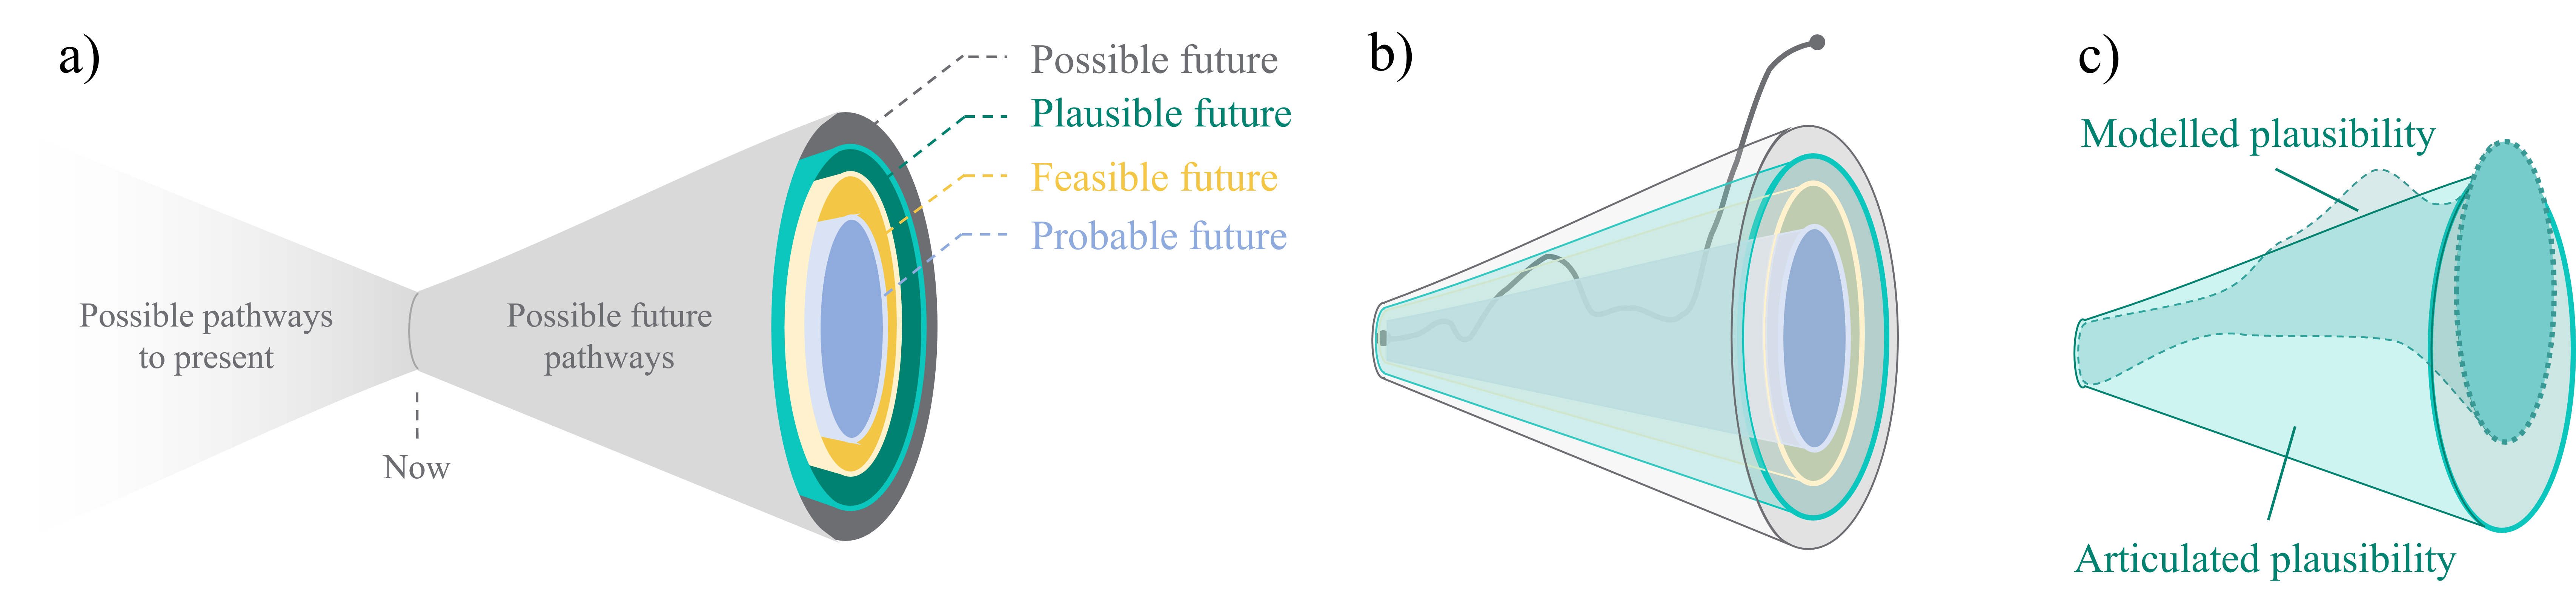
\includegraphics[width=\textwidth]{Cones_plausibility.png} 
    \caption[Some caption for list of figures]{Scenario cones for a variable of interest. a) Multiple alternative futures are possible, which may be narrowed down through the use of qualifiers. b) Extreme events may lie outside of what we currently consider possible. c) Scenarios depend on models and (explicit or implicit) storylines (=ideas of the future), both of which may be qualified in terms of their plausibility, which is not necessarily congruent. 
    Source: 1.a) Adapted from Jewell and Cherp \url{https://wires.onlinelibrary.wiley.com/doi/10.1002/wcc.838}, 1.b) adapted from McCollum et al. \url{https://www.nature.com/articles/s41560-020-0555-3}, 1.c) own elaboration.}  
    \label{fig:plausibility}
\end{figure}

\subsection{Sustainability scenario models}

Models are only abstract representations of our world, and socio-ecological systems are too complex to be adequately represented by only a single model. 
Choices along the development and use of a model introduce thus ambiguity, which amplifies when expanding the system boundary from past and present to the future. 
Indeed, a great many families of sustainability models are available, including those for environmental management (\url{https://www.sciencedirect.com/science/article/pii/S1364815213001151?via%253Dihub}) and socio-metabolic research \parencite{haberl_2019}. 
Many of these models and methods are increasingly being adapted and used for prospective analyses, in particular for scenario exercises.

Today's sustainability scenario-modelling is largely dominated by the integrated assessment modelling community, their models, and the scenarios that they develop. 
Integrated assessment models (IAMs) can be classified either as cost-benefit or process-based models: 
the former are in direct lineage of Ronald Coase's concept of social cost and most often are highly aggregated models, whereas most process-based models emerged from the literature on energy modelling and are comparatively detailed.\footnotemark{} 
Cost-benefit models such as PAGE \parencite{yumashev_2019}, FUND \parencite{waldhoff_2014}, and DICE/RICE \parencite{nordhaus_2017} are sometimes also termed policy optimisation models and typically employed to identify the \textit{optimal} balance (based on some criterion) between costs and benefits of policies and impacts. 
Process-based models such as IMAGE \parencite{stehfest_2014}, MESSAGE \parencite{huppmann_2019}, and REMIND \parencite{baumstark_2021} are often referred to as policy evaluation models.
They are used to evaluate socio-economic and environmental consequences of actions and impacts; 
depending on their level of integration and system representation, process-based models are sometimes also referred to as energy-economy-environment (E3) or E4 (E3 + engineering) models. 
Some models, such as WITCH \parencite{bosetti_2006,emmerling_2016}, can be employed for both policy optimisation and evaluation.

\footnotetext{\textcite{nikas2019,hafner2020} provide alternative detailed classifications of IAMs.}

Scenario sets originating from the (process-based) IAM community are highly authoritative and form an important basis for global decision-making with regard to climate and other environmental change (e.g. \url{https://doi.org/10.1016/j.gloenvcha.2020.102191}). 
Such scenario sets include in particular the representative concentration pathways \parencite[RCPs;][]{vanvuuren_2011_rcp} and the shared socio-economic pathways \parencite[SSPs;][]{riahi_2017,oneill_2014} in the context of climate change. 
Comprehensive scenario sets for the wider sustainability perspective are less common \parencite{vansoest_2019}, but include notably the sustainable development pathways developed by The World in 2050 initiative \parencite{twi_2018}. 
Modelling approaches from other domains of sustainability science often adopt the assumptions, input parameters, or scenario outputs from these authoritative sources.

Yet, IAMs are not without their flaws and have therefore been criticised repeatedly. 
Because of prominent role of IAMs in sustainability scenario modelling, we want to briefly touch upon these. 
Perceived failings and problematic aspects include excessive techno-optimism (\url{https://www.science.org/doi/10.1126/science.aah4567}), incomplete exploration of the possibility space \parencite{keppo_2021,mccollum_2020, gambhir_2022}, arbitrary functional forms \parencite{pindyck_2017}, ignorance towards uncertainty \parencite{stern_2016}, application of discount rates \parencite{emmerling_2019}, disregard for emerging behaviours \parencite{farmer_2015}, and unrealistic behavioural assumptions \parencite{asefi_2021}. 
However, not all criticisms are valid for each IAM. 
After all, there are great differences among IAMs in terms of model structures, input assumptions, and model outcomes \parencite{krey_2014,krey_2019,hiroto_2020,keppo_2021}. 
This, in turn, may hamper model comparisons \parencite{giarola_2021,sognnaes_2021} as one would not want to end up comparing apples and oranges.

The spawn of IAMs (rooted in energy modelling) in the second half of the ${20}^{th}$ century coincided with sustainability concerns seeping into other scientific disciplines: 
For example, in Earth Science, Earth system models expanded from modelling only biogeochemical processes of the Earth system to also account for human drivers of changes \parencite{flato_2011}; 
the engineering discipline brought forth the field of industrial ecology \parencite{frosch_1989,ausubel_1992,jelinski_1992}; 
and ecological economics emerged from the dismal science \parencite{cleveland_1999}. 
Thus, one may observe today a large heterogeneity of models and model families used to analyse socio-ecological systems. 
These differ not only in their origins and traditions, but also in terms of the aspects they focus on and their underlying principles. 
For example, IAMs often do not explicitly represent society's biophysical basis, while this is essential to industrial ecology approaches \parencite{pauliuk_2017}. 
And while industrial ecology and ecological economics share assumptions and considerations, their detail of analysis often differs \parencite{kronenberg_2006}. 
In addition, one can identify even within model families large differences, such as regarding solution concepts in IAMs or the scale of analysis in industrial ecology.

Increasingly, non-IAM sustainability models are used for scenario analyses, too. 
Next to standalone non-IAM sustainability scenario models, IAMs and non-IAM models are often integrated (e.g. IAMs and input-output models \url{https://doi.org/10.1080/09535314.2023.2266559} or lifecycle assessment models \url{https://doi.org/10.1007/s11367-021-01954-6}), although the degree of integration can vary: 
the models can either be hard-coupled, soft-coupled, or information may flow uni-directionally. 
When sustainability scenario models are integrated with others or when they adapt or customise existing parameterised scenarios, 

\subsection{Aspects of scenario planning}

But what are scenarios actually? 
Spaniol and Rowland on defining "scenario" \url{https://onlinelibrary.wiley.com/doi/10.1002/ffo2.3} and a response by Chermack \url{https://onlinelibrary.wiley.com/doi/full/10.1002/ffo2.13}, supporting many points made but also objecting others, e.g. that scenarios need narratives.

Scenario planning vs overlap of foresight/forecast/planning

Elsawah et al. on the scenario process \url{https://www.sciencedirect.com/science/article/pii/S0048969720319069}. Peterson et al also describe a scenario process \url{https://conbio.onlinelibrary.wiley.com/doi/10.1046/j.1523-1739.2003.01491.x}

Distinguish scenarios from counterfactuals as Booth et al. do \url{http://dx.doi.org/10.1016/j.futures.2008.07.037}. Both are types of modal narratives, but while scenarios are future-oriented, counterfactuals refer to the past (with what-if questions)

Various scenario typologies exist, a popular one being the one by Börjeson et al. Bishop et al. on scenario typologies and similar \url{https://www.emerald.com/insight/content/doi/10.1108/14636680710727516/full/pdf?title=the-current-state-of-scenario-development-an-overview-of-techniques}. Other typologies and classifications are provided/summarised by Amer et al. \url{https://www.sciencedirect.com/science/article/pii/S0016328712001978}, or earlier by van Notten et al. \url{https://www.sciencedirect.com/science/article/pii/S0016328702000903}

Related to that, have a look at the scenario intervention typology by Crawford \url{https://www.sciencedirect.com/science/article/pii/S0040162519306924?via%3Dihub}

Cuhl on the distinction between foresight, forecasting, planning \url{https://doi.org/10.1002/for.848}; scenarios as part of foresight

Lazurko: "The scenario process occurs in the present
and involves boundary judgments that delimit the scope of future
potential (i.e., future conditions and values) reflected in the resulting
scenarios." therefore need for qualifiers as well as proper framework to apply them
We understand reflexivity here as the critical reflection of how design and use of models and scenarios influence their outcomes and impact.

Although predictions of such complex systems as the human and natural systems are practically impossible, other ways of addressing the future have been devised \parencite{polasky_2011}, with scenario-modelling being now well-established in sustainability science.

\subsubsection{Scenario elements}
Assumptions, beliefs, ideas, emotions, values, norms...
..a collection of assumptions, beliefs, expectations etc of an individual or group, referred to here as worldview. 
We acknowledge that the term worldview may be used differently in some disciplines.
(de Vries and Petersen define worldviews as: "being combinations of value orientations and world interpretations, at the individual level." \url{https://www.sciencedirect.com/science/article/pii/S0921800908005016}

Observations, expectations, imaginaries, narratives \url{https://journals.sagepub.com/doi/full/10.1177/00380385221138010#fn2-00380385221138010}

Scenario inputs (data, models, narratives etc) and outputs, processes, and objectives \url{https://www.annualreviews.org/doi/full/10.1146/annurev-environ-112321-095011}


\subsubsection{The scenario process}
Scenario equation by Uruena, but perhaps include also another process (in addition to inferential ones) since inferential ones don't help much wrt extreme events and unknown unknowns. Uruena mentions also imaginative reasoning (complimentary to abductive reasoning)

Ambiguity of scenario processes makes use of plurality of models (therefore sets of models) necessary

Below equations are rooted in the present, therefor (e) does not need time index. However, it's worth a thought that at other points in time, (e) would be different and thus affecting how and what kind of model or scenario is developed.
\begin{align}
        &{S}^{L}_{t} + \{e\} \rightarrow \{{S}^{L}_{f}\}, \label{eq:scenario_qualitative}\\
        &{S}^{N}_{t} + \{e\} \rightarrow \{M\} = \{\{{M}^{C}\}, \{{M}^{A}\}\}, \label{eq:model_generation}\\
        &\mathcal{S} + \{e\} + m \rightarrow \{{S}^{N}_{f}\},\ \text{if}\ \exists\ {S}^{N}_{\bullet} \in \mathcal{S}, \label{eq:scenario_quantitative}\\
        &\mathcal{S} \subset \bigcup \{{S}^{\bullet}_{\bullet}\},\ m \in \{M\}. \label{eq:state_set}
\end{align}


\subsubsection{A jungle of scenario qualifiers}
Possibility, probability, likeliness, plausibility, feasibility, desirability, consistency, contingency.

Uruena as prime source on meaning and role of plausibility \url{https://www.sciencedirect.com/science/article/pii/S0016328718303264?via%3Dihub} Fischer and Dannenberg might continue along these lines \url{https://www.sciencedirect.com/science/article/pii/S0016328721000380?via%3Dihub} and Glette-Iversen in the risk context \url{https://www.sciencedirect.com/science/article/pii/S0925753521004756?via%3Dihub}; Glette-Iversen provide a list of plausibility definitions found in literature and classify them into two groups - Uruena's definition combines these groups.

Ramirez and Selin on the distinction between plausibility and probability \url{https://www.emerald.com/insight/content/doi/10.1108/FS-08-2012-0061/full/html}. (Interestingly, they actually question the depiction of the future as a cone... maybe I should mention in the figure caption that the shape was arbitrarily chosen to be conic but that in reality it may take any shape)

Wiek et al. are an important references as well \url{https://www.researchgate.net/profile/Lauren-Keeler/publication/263276841_Plausibility_indications_in_future_scenarios/links/573b616508ae9ace840ea713/Plausibility-indications-in-future-scenarios.pdf}

Futures pyramid by Dorsser et al. \url{https://www.sciencedirect.com/science/article/pii/S0016328717302513?via%3Dihub}

Walton et al. on "theory of plausibility" with case study in New Zealand \url{https://www.sciencedirect.com/science/article/pii/S0016328718300892?via%3Dihub#bib0375}

Schmidt-Scheele discusses how users of scenarios assess their plausibility \url{https://www.sciencedirect.com/science/article/pii/S2211467X20301243?via%3Dihub#bib24}

Fischer and Dannenberg on plausibility, emphasising many of Uruena's points \url{https://doi.org/10.1016/j.futures.2021.102729}

Janasik again on plausibility vs probability \url{https://www.sciencedirect.com/science/article/pii/S0016328720301609?via%3Dihub}

Plausibility in IAMs via fiction, by van Beek and Versteeg \url{https://www.sciencedirect.com/science/article/pii/S001632872300099X?via%3Dihub}

In 2.2.8, van Vuuren et al. refer to scenario classifiers (=qualifiers?): saliency, credibility, legitimacy \url{https://www.sciencedirect.com/science/article/pii/S0959378012000635}

Walton et al. developing a theory of plausibility in scenario building \url{https://doi.org/10.1016/j.futures.2019.03.002}

Vervoort et al. might provide some good recap of existing divide regarding probability (positivist camp) and plausibility (constructivist camp (post-normal?)) \url{https://www.sciencedirect.com/science/article/pii/S0016328715001184}

Another view on plausibility by Hajer and Pelzer? \url{https://www.sciencedirect.com/science/article/pii/S2214629618300732}

Robertson on transparency in IPCC modelling \url{https://wires.onlinelibrary.wiley.com/doi/full/10.1002/wcc.679}

Braunreiter et al. argue that scenarios should support rather than narrow down deliberations on possible and desirable futures \url{https://www.sciencedirect.com/science/article/pii/S2214629621003133}

Schmidt-Scheele on plausible energy scenarios \url{https://www.sciencedirect.com/science/article/pii/S2211467X20301243}

Jewell and Cherp on feasibility spaces \url{https://wires.onlinelibrary.wiley.com/doi/10.1002/wcc.838}

\subsubsection{Opening up and closing down futures}
Explain why plausibility is a better criterion than the too-vast possibility and the conditional (because based on past and present trends into the unknown future) probability

Plausibility as an epistemic device, scenarios as perception devices (uruena). He also argues that plausibility requires an additional identifier/criterion.

Plausibility used in the scenario creation process and as a criterion for evaluating a scenario. (Uruena describes this as methodological-delimiting and anticipatory-enabling.) I guess one might add that plausibility could also be added as a criterion in the model generation process (if validation is not or only at high costs possible)
Moreover, in terms of using plausiblity as a criterion for evaluating scenarios, it is important to consider that very heterogenous user groups may use the constructed scenarios, but were maybe not involved in the scenario construction process. These users might therefore be confronted with a large number of different and potentially contradicting scenarios such that they have to evaluate their plausibility differently (+ by different means) from how users would who were engaged in the construction process. See book by Schmidt-Scheele \url{https://www.degruyter.com/document/doi/10.1515/9783839453193/html?lang=en}. In that book, the author also shows that users rate scenarios' plausibility according to source credibility, i.e. who constructed the scenarios, and according to how likely the scenarios appears to be, i.e. it is based on individual beliefs and expectations... I assume many of her points are also contained in her paper \url{https://www.sciencedirect.com/science/article/pii/S2211467X20301243}

At the same time, plausibility is subjective. Would pre-cautionary approaches admonish us to think BIG and thus consider rather possibility?
At the same time, some have argued that applying precautionary approaches requires the identification of plausible threats...
Tipping points are of course of more uncertain nature, but other climate impacts and other environmental impacts more generally are more certain



\subsection{Possibility, solution, and target spaces: where is the future?}

Define possibility space, solution space, and target space.

Also mention "scenario space" as Braunreiter et al did (\url{https://doi.org/10.1016/j.erss.2021.102220})

On target space (of SDGs) \url{https://www.cell.com/one-earth/pdf/S2590-3322(22)00003-3}

Keppo et al. on exploring the possibility space; basically a review of and response to criticisms towards IAMs (\url{https://iopscience.iop.org/article/10.1088/1748-9326/abe5d8})

Scenarios are more than continuations of past legacy.

Future path dependency depends on past, present, and future decisions. Future path dependency does not continue right from present path dependency - the time in between matters and may feature creative and other disruptions. Therefore, plausibility is time-contingent.

Talk about black swans as well as grey swans / dragon kings and grey rhinos. 
(And with that also talk about regime changes, (social + natural) tipping points etc.)
An evaluation of alleged black swan events \url{https://www.sciencedirect.com/science/article/pii/S0013935120300190}


\begin{figure} [ht]
    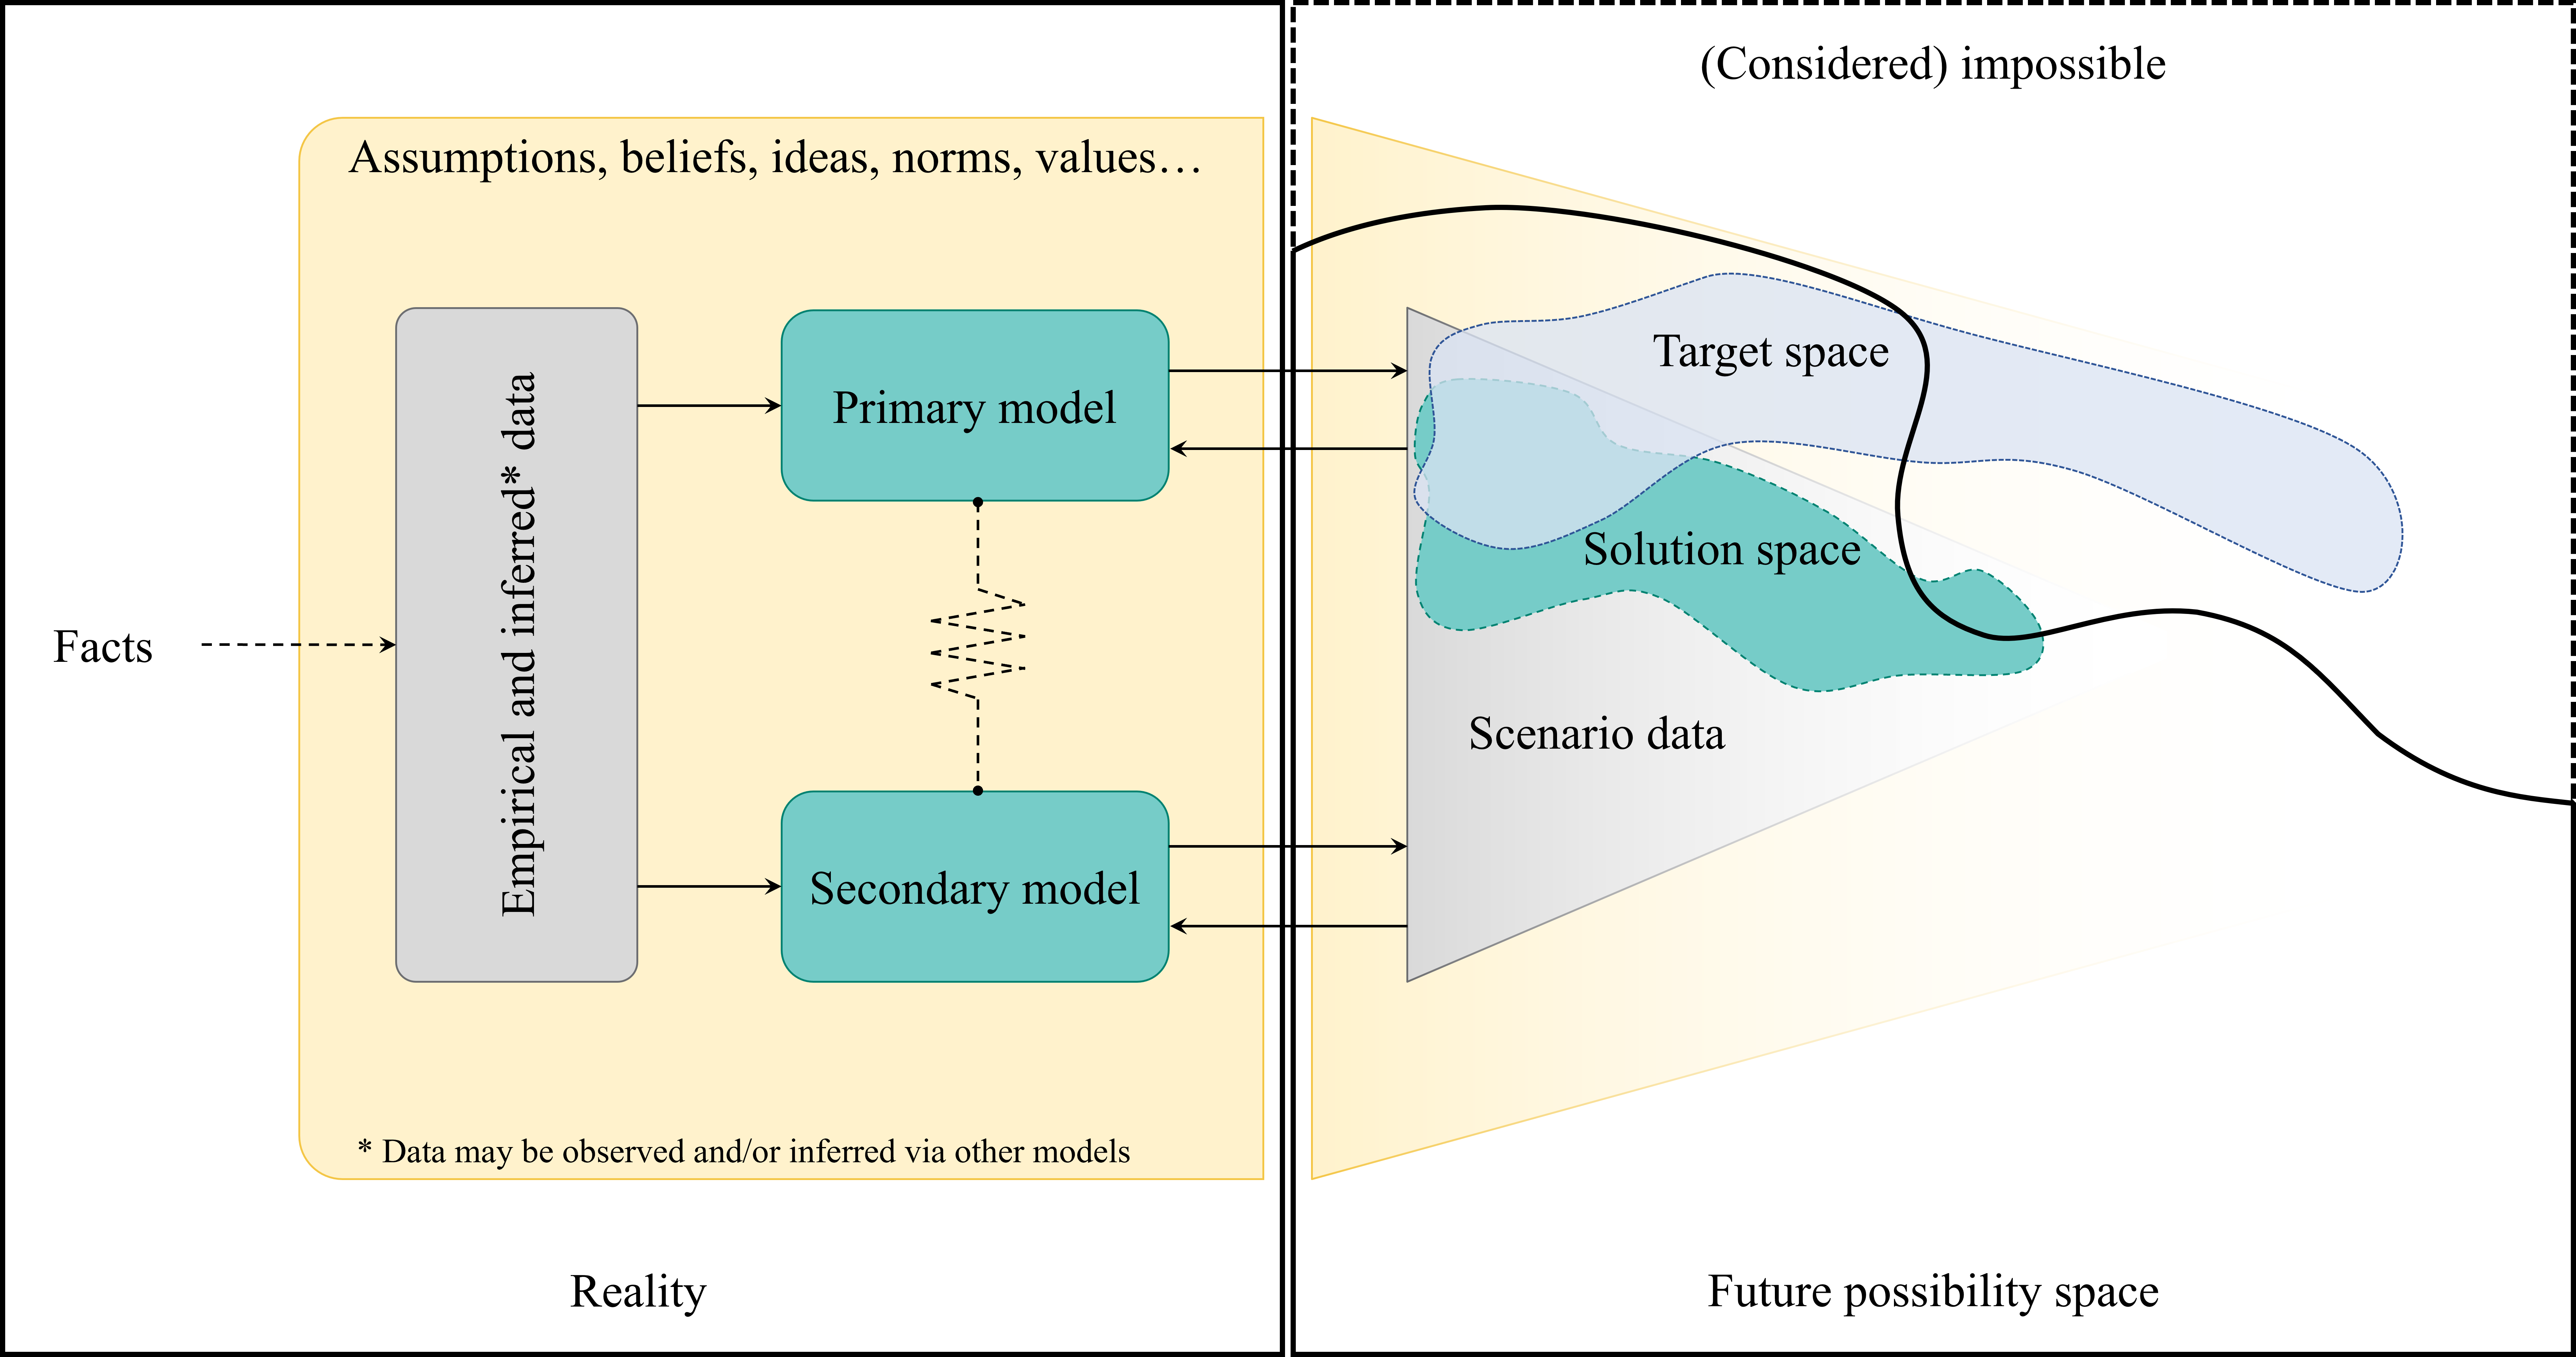
\includegraphics[width=\textwidth]{Model_spaces.png} 
    \caption[Another caption for list of figures]{Models use and produce data and may influence each other. The future consists of different spaces, which may differ dependent on which model is used.}
    \label{fig:model_spaces}
\end{figure}


\label{main_part}
\section{Positionality, reflexivity, and interdependency}

Basically reiterate many of the points made by Lazurko et al. but apply to the present case, i.e. when models inform each other (via coupling or not)

Add my points on primary and secondary models. Supported by figure 2. 
Primary models being primarily IAMs, and secondary models for example IE models. Another way of seeing it is that primary models are causal/dynamic models, and secondary models are attributional models. Or: primary models are those with which authoritative scenario sets are created, and secondary models are those which use (adapt/customise) these scenarios then.

Idea behind figure: 
Reality provides facts. 
Facts are observed (therefore data) and shape our assumptions beliefs, norms etc. 
Our assumptions etc. determine in turn which data we collect. 
Generally, reality and our assumptions, beliefs, norms etc. are constantly in interaction via inferential (= inductive, deductive, and abductive) processes. 
Existing data are used as inputs for primary and secondary models. 
These models can be coupled, either hard or soft - or not at all. 
--
We also have assumptions etc about the future. 
These assumptions etc. form, however, only a subspace of the full possibility space. 
At the same time, our assumptions etc. shape the possibility space. 
Primary and secondary models may be used for scenario modelling, generating and potentially also using scenario data. 
Scenario data consists of exogenous and endogenous halves. The exogenous part is determined by our assumptions etc. about the future whereas endogenous part is determined through the model (which is based on past/current data and/or assumptions etc.). 
Often, scenario data generated with primary models is used for further analysis with secondary models, with conflicts of assumptions and ambiguities being a possible result. 
The solution space contains those parts of the scenario data which were/could be computed for a given single scenario. 
Target space describes what is desirable in terms of targets. 
We might have some targets that lie outside of what can be examined with the models (target space outside of solution space). 
Some targets may be impossible, e.g. because various targets are conflicting. 
We have assumptions about what the future could be like, but that future might simply not be possible.

Our exploration regards in particular the cases when the interaction between primary and secondary models is of a soft-coupled or selective-data-adoption nature, which may often be the case when existing large-scale (e.g. global) scenario sets are downscaled.

\begin{figure} [ht]
    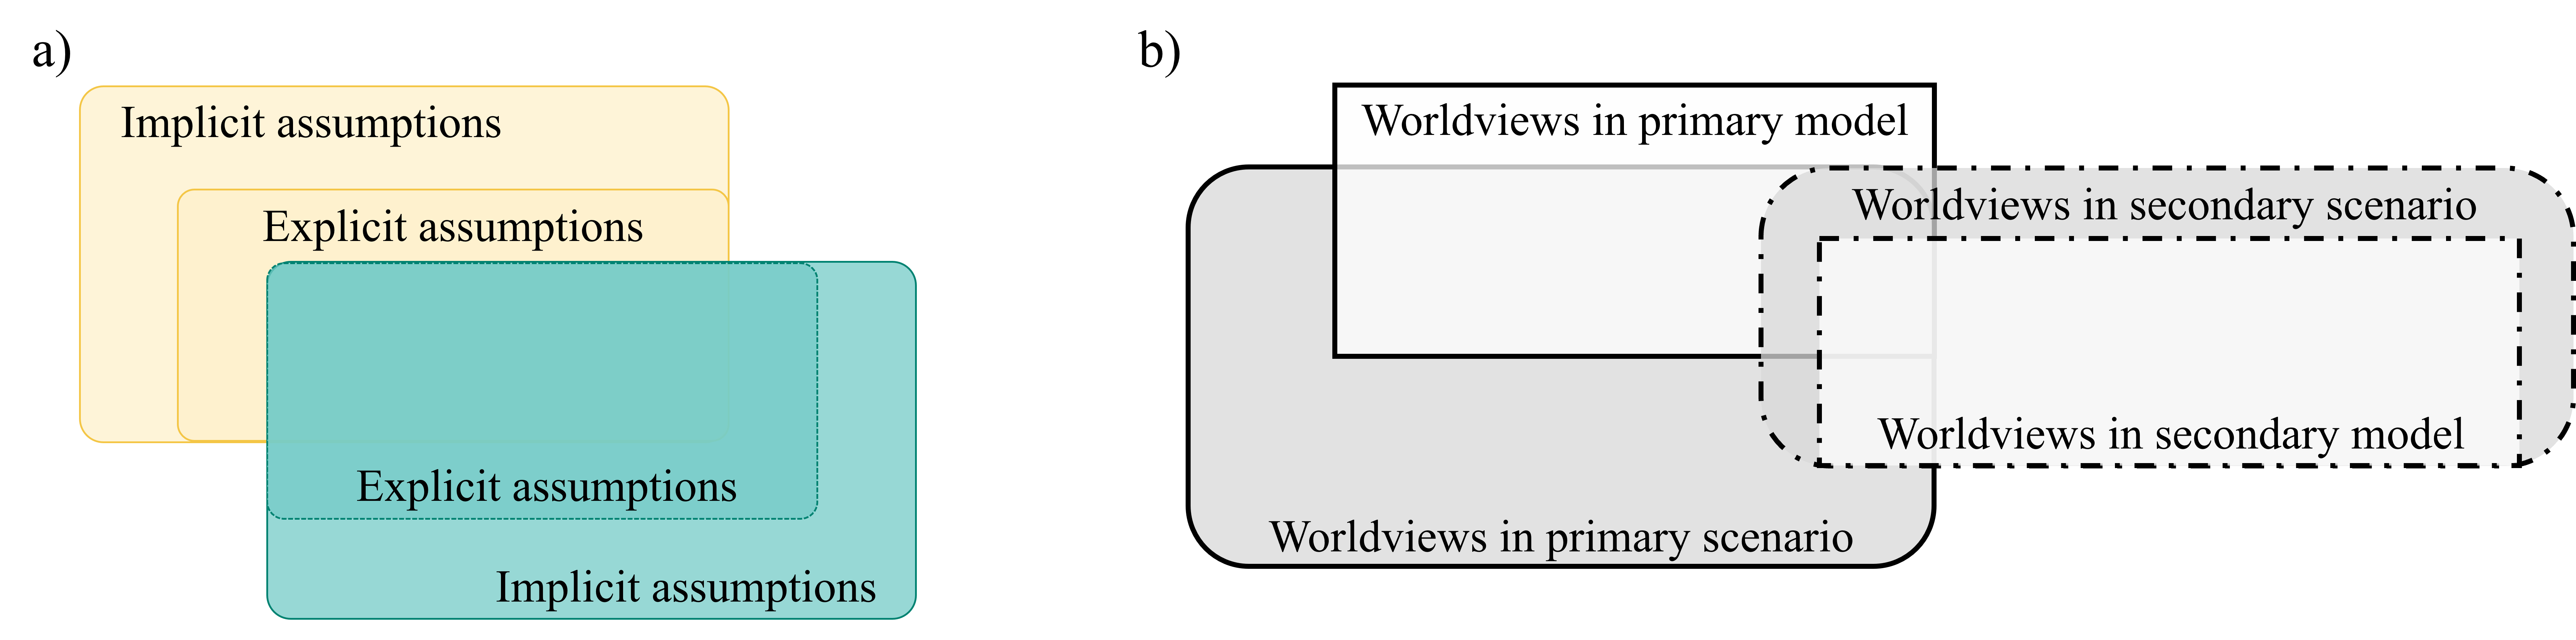
\includegraphics[width=\textwidth]{Worldviews.png} 
    \caption[Some caption for list of figures]{a) An artefact (such as a scenario or model) is characterised by explicitly formalised/formulated assumptions as well as by conditions and contexts implied by the former. The (explicit or implicit) assumptions underlying one artefact might not be congruent with those of another (as indicated by the different colours). b) The worldviews contextualised in a qualitative scenario may differ from those embedded (explicitly and implicitly) in a quantitative model used for modelling said scenario (as indicated for primary model and scenario). Likewise, the worldviews underlying a secondary modelling exercise may not be fully congruent, coherent, or consistent with those of a to-be-used (primary) parameterised scenario. For both a) and b), the overlaps of elements are only illustrative and not be understood as the general case; for example, it may well be that the explicit assumptions of two artefacts align or that the worldviews underlying a primary and a secondary modelling exercise are consistent.}  
    \label{fig:worldviews}
\end{figure}

"either the process of developing the scenarios can be connected or the elements and outcomes of the scenarios can be linked (Zurek and Henrichs 2007)" in Biggs et al. \url{https://www.ecologyandsociety.org/vol12/iss1/art17/}; Zurek and Henrichs \url{https://doi.org/10.1016/j.techfore.2006.11.005}

Adapting and customising scenarios with secondary models naturally leads to continuing someone else's model-land (\url{https://www.degruyter.com/document/doi/10.5018/economics-ejournal.ja.2019-40/html}), a situation in which reflexivity practice (Luzarko et al.) can help reduce ambiguities and inconsistencies. (Some ambiguities and inconsistencies might remain, e.g. some assumptions remaining hidden no matter what as McDowall and Geels pointed out \url{https://doi.org/10.1016/j.eist.2016.07.001})

Someone's plausible scenario output might be someone else's implausible scenario input (and vice versa)

Today's sustainability scenario-modelling is largely dominated by the IAM community, their models, and the scenarios that they develop. While the development process for the most authoritative global change scenarios has evolved from moving only sequentially along the causal chain to a more parsimonious, parallel process \parencite{moss_2010} and ultimately combining scenario sets in a matrix architecture \parencite{vanvuuren_2014},\footnotemark{} SSPs rely just like RCPs (and often other frameworks, too) on marker scenarios. That is, for each of a set of agreed upon narratives there is one representative scenario implementation chosen. Non-marker scenarios can then be understood as alternative scenario interpretations \parencite{riahi_2017}. The marker scenarios are, however, the authoritative ones and are exclusively implementations made with major IAMs such as AIM \parencite{fujimori_2017}, GCAM \parencite{calvin_2017}, and MESSAGE \parencite{fricko_20171}. When such scenarios are then taken over by other assessment methods, it is usually only the marker scenarios that are employed, thus introducing a bias towards the bigger IAMs (and thus towards large modelling teams that might also receive comparatively more funding). Also across different scenario sets, there is a bias towards larger IAMs: among all 1,686 vetted pathways explored in the IPCC Sixth Assessment Report database using a pool of more than 20 models, about one third was computed using MESSAGE and REMIND \parencite{gambhir_2022,byers_2022}.
\footnotetext{Although many goals were achieved with this scenario architecture, the common sentiment among respective modellers is that further improvements must be made, such as the integration of societal conditions \parencite{oneill_2020}. Others have raised their voices concerning the plausibility of some scenario combinations, such as SSP3-RCP7.0 or RCP5-SSP8.5 \parencite{pielke_2022}.}

Differentiate between scenario adaptation and/or customisation and ignorant use of numbers. This review could be useful \url{https://www.annualreviews.org/doi/full/10.1146/annurev-environ-102017-030109}

\section{Moving forward}

Recap + recommendation + conclusion

\begin{itemize}
    \item provide guidance on how reflexivity practice could be adopted by secondary modellers. At least, the use of scenario qualifiers needs to be adopted.
    \item secondary modelling should explore the existing possibility space more comprehensively (e.g. by not only taking SSP marker scenarios as inputs).
    \item extreme events need to be explored more comprehensively. Perhaps include "dummy extreme events", i.e. possible disruptions of some parameters along the way (at some time step), perhaps even "compund extreme events" (which may push the actual pathway far from what is currently considered plausible). Similarly, create perhaps a "very worst case" scenario where all such possible disruptions happen (applied to all parameters)
    \item for both primary and secondary modelling: reduce sectoral (+spatiotemporal) resolution when further in the future
\end{itemize}

\newrefcontext[sorting=nyt] % sort the paper by name, year, title
\printbibliography[heading = bibintoc] % 'bibintoc' inserts our bibliography into the table of contents

\end{refsection}

%%%%%%%%%%%%%%%
%% Appendix
%% Inserting appendix with separate settings
%\newpage
%\setcounter{page}{1}
%\renewcommand{\thepage}{A-\arabic{page}}
%\linenumbers*
%\addappendix
%
%%Reset numbering of tables and equations in appendix, starting with A.
%\renewcommand{\thetable}{A.\arabic{table}}
%\setcounter{table}{0}
%\renewcommand{\theequation}{A.\arabic{equation}}
%\setcounter{equation}{0}
%
%\begin{refsection}
%\section*{Appendix A}
%BLABLA
%
%\section*{Appendix B}
%blabla
%
%\nolinenumbers
%\newpage
%\newrefcontext[sorting=nyt] % sort the paper by name, year, title
%\printbibliography[title = References in appendix]
%
%\end{refsection}
\end{document}